%PS_subsequences_partial_order_Dilworth_Lemma

\documentclass[problem]{mcs}

\begin{pcomments}
  \pcomment{from: F07.ps2}
\end{pcomments}

\pkeywords{
  subsequences
  maximum_length_of_subsequences
  partial_order
  maximal_and_minimal_elements
  Dilworth_Lemma
}

%%%%%%%%%%%%%%%%%%%%%%%%%%%%%%%%%%%%%%%%%%%%%%%%%%%%%%%%%%%%%%%%%%%%%
% Problem starts here
%%%%%%%%%%%%%%%%%%%%%%%%%%%%%%%%%%%%%%%%%%%%%%%%%%%%%%%%%%%%%%%%%%%%%

\begin{problem}
Let $S$ be a sequence of $n$ different numbers.  A \term{subsequence} of
$S$ is a sequence that can be obtained by deleting elements of $S$.

For example, if
\[
S = (6,4,7,9,1,2,5,3,8)
\]
Then $647$ and $7253$ are both subsequences of $S$ (for readability, we
have dropped the parentheses and commas in sequences, so $647$ abbreviates
$(6,4,7)$, for example).

An \term{increasing subsequence} of $S$ is a subsequence of whose
successive elements get larger.  For example, $1238$ is an increasing
subsequence of $S$.  Decreasing subsequences are defined similarly; $641$
is a decreasing subsequence of $S$.


\begin{problemparts}

\problempart  
List all the maximum length increasing subsequences of $S$, and all
the maximum length decreasing subsequences.

\begin{solution}
The maximum length increasing subsequences are $1238$ and
$1258$.  The maximum length decreasing subsequences are
\[
641, 642, 643, 653, 753, 953
\]
\end{solution}

\end{problemparts}

Now let $A$ be the \emph{set} of numbers in $S$.  (So $A =
\set{1,2,3,\dots,9}$ for the example above.)  There are two
straightforward ways to totally order $A$.  The first is to order its
elements numerically, that is, to order $A$ with the $<$ relation.  The
second is to order the elements by which comes first in $S$; call this
order $<_S$.  So for the example above, we would have
\[
6 <_S 4 <_S 7 <_S 9 <_S 1 <_S 2 <_S 5 <_S 3 <_S 8
\]

\iffalse
letting $a_i$ be the $i$th element of $S$, we order $A$ with the total
order $<_S$, where
\[
a_i <_S a_j \iff i < j.
\]
\fi

Next, define the partial order $\prec$ on $A$ defined by the rule
\[
a \prec a' \quad \eqdef \quad a  < a' \text{ and } a <_S a'.
\]
(It's not hard to prove that $\prec$ is strict partial order, but you may
assume it.)


\begin{problemparts}

\problempart 
Draw a diagram of the partial order, $\prec$, on $A$.  What are the
maximal elements,\dots the minimal elements?

\begin{solution}
The maximal elements are 8 and 9; the minimal are 1, 4,and 6:
\begin{center}
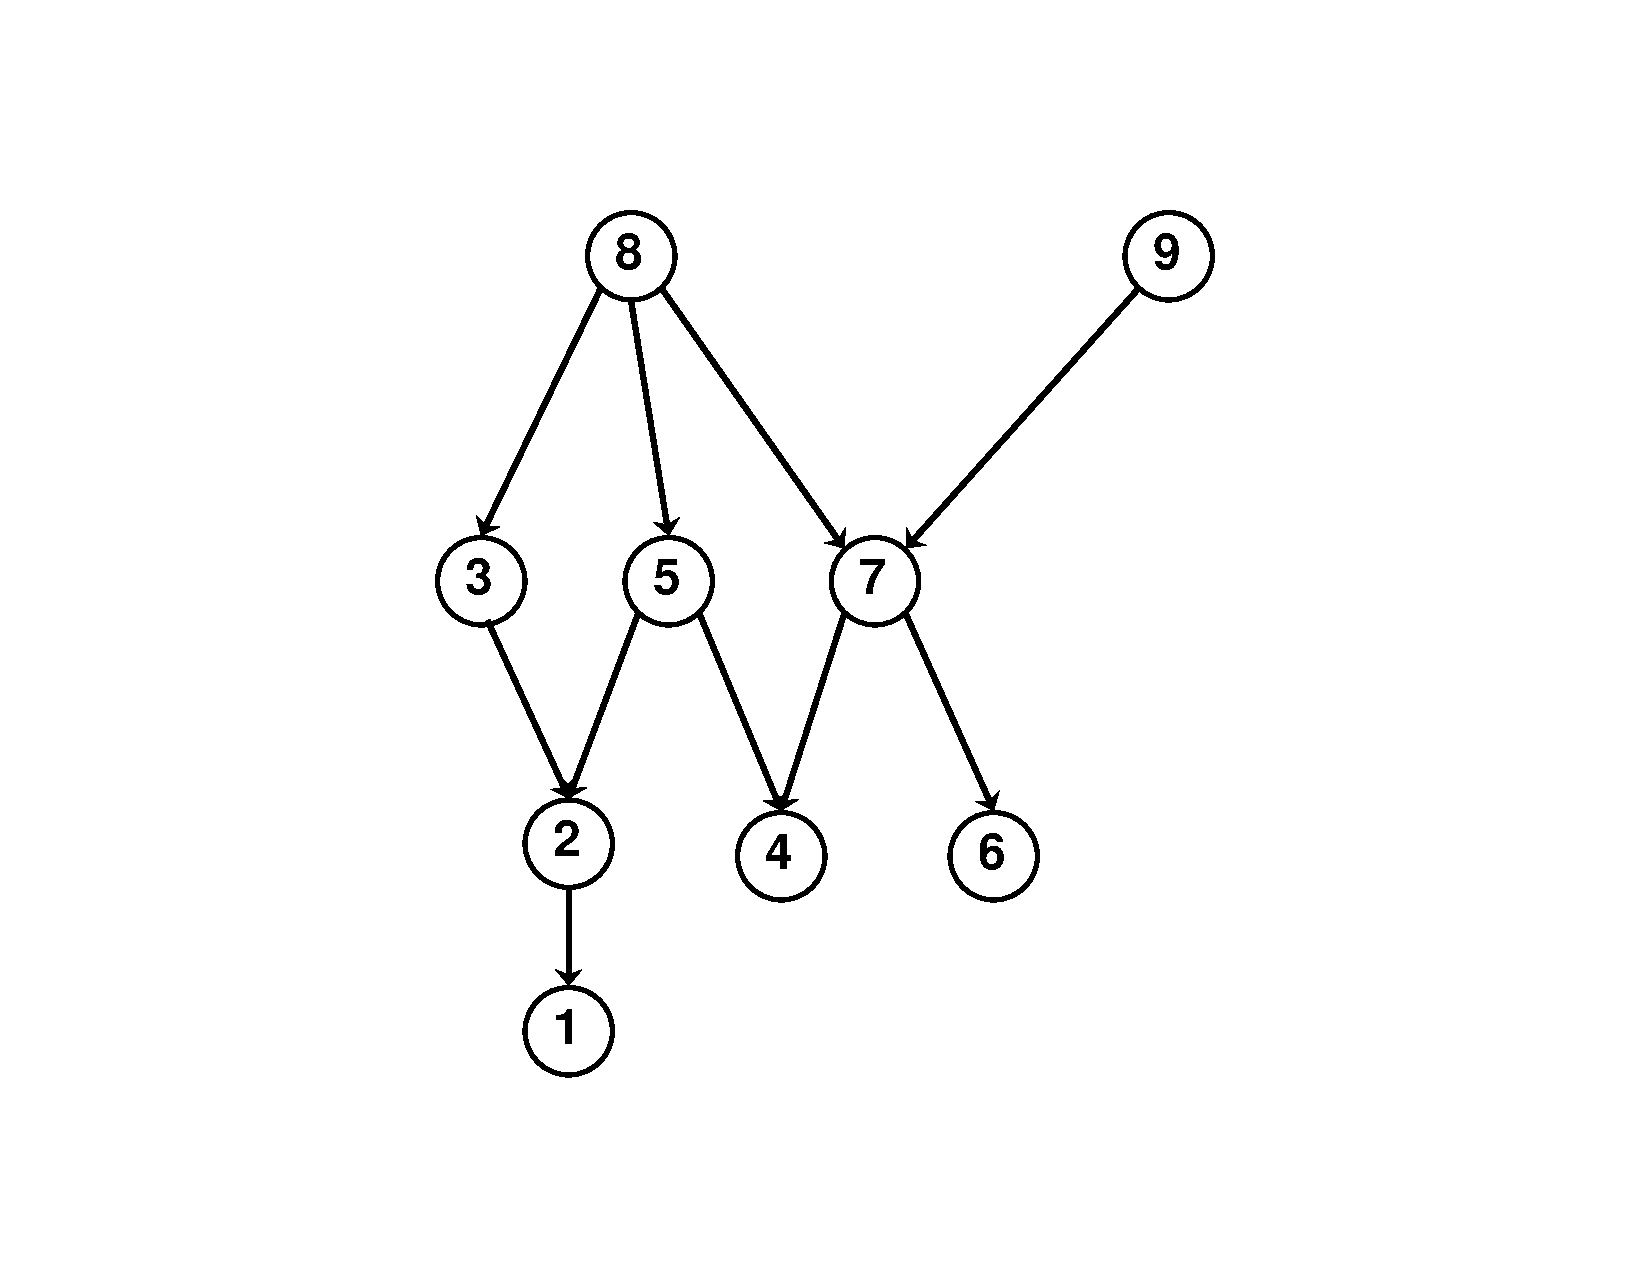
\includegraphics[height=4in]{figures/sequence-poset.pdf}
\end{center}
\end{solution}


\problempart
Explain the connection between increasing and decreasing
subsequences of $S$, and chains and anti-chains under $\prec$.

\begin{solution}
A \emph{chain}, with its elements listed in numerically
increasing order, is an \emph{increasing} subsequence and an
\emph{antichain}, with its elements listed in numerically decreasing
order, is a \emph{decreasing} subsequence.
\end{solution}


\problempart 
Prove that every sequence, $S$, of length $n$ has an increasing
subsequence of length greater than $\sqrt{n}$ or a decreasing subsequence
of length at least $\sqrt{n}$.
\iffalse

\hint
\href{http://courses.csail.mit.edu/6.042/fall07/ln3.pdf#rule.Dilworth}
{Dilworth's Lemma}
\fi

\begin{solution}
By Dilworth's Lemma, either a chain or an antichain must have
size at least $\sqrt{n}$, which, by the previous problem part, means there
is either an increasing or a decreasing subsequence of this size.  
\end{solution}

\ppart (Optional, tricky) Devise an efficient procedure for finding the
longest increasing and the longest decreasing subsequence in any given
sequence of integers.  (There is a nice one.)

\begin{solution}
\TBA{reference to Floyd algorithm}
\end{solution}

\end{problemparts}

\end{problem}

%%%%%%%%%%%%%%%%%%%%%%%%%%%%%%%%%%%%%%%%%%%%%%%%%%%%%%%%%%%%%%%%%%%%%
% Problem ends here
%%%%%%%%%%%%%%%%%%%%%%%%%%%%%%%%%%%%%%%%%%%%%%%%%%%%%%%%%%%%%%%%%%%%%

\endinput
